\PassOptionsToPackage{xetex}{xcolor}
\PassOptionsToPackage{xetex}{graphicx}
\documentclass[a4paper,landscape,headrule,footrule,xetex]{foils}

%%
%%%  Macros
%%%
\newcommand{\logo}{~}
\MyLogo{HG2052 (2020)}
%\newcommand{\Story}{\SHA{HOUN}{The Hound of the Baskervilles}}

\newcommand{\header}[3]{%
\title{\vspace*{-2ex} \Large HG2052
\\\large  Language, Technology and the Internet
\\[2ex] \Large  \emp{#2}}
\author{\blu{Francis Bond}   \\ 
\normalsize  \textbf{Division of Linguistics and Multilingual Studies}\\
\normalsize  \url{http://www3.ntu.edu.sg/home/fcbond/}\\
\normalsize  \texttt{bond@ieee.org}}
\MyLogo{HG2052 (2020)}
\date{#1}
\renewcommand{\logo}{#2}
 \hypersetup{
   pdfinfo={
     Author={Francis Bond},
     Title={#1: #2},
     Subject={HG2052: Language, Technology and the Internet},
     Keywords={Language, Technology, Internet},
     License={CC BY 4.0}
   }
 %  pdfcopyright={Copyright © Francis Bond. Creative Commons 4.0 Attribution License.}
 %  pdflicenseurl={http://creativecommons.org/licenses/by/4.0/}
 }
}


%%
%% Multilingual Stuff
%%
\usepackage[a4paper,landscape,margin=25mm]{geometry}

\usepackage{fontenc}
\usepackage{polyglossia}
\setmainlanguage{english}
\setmainfont{TeX Gyre Pagella}
%\setmainfont{Linux Libertine}
%\setmainfont{Charis SIL}
\newfontfamily{\ipafont}{Gentium}
\newcommand{\ipa}[1]{{\ipafont\selectfont #1}}
\usepackage{xeCJK}

\setCJKmainfont{Noto Sans CJK SC}
\setCJKsansfont{Noto Sans CJK SC}
%\setCJKttfont{Noto Sans CJK SC}
%\setCJKmainfont{WenQuanYi Micro Hei}
%\clearpage
%\setCJKmainfont{AR PL SungtiL GB}

\usepackage[xetex]{xcolor}
\usepackage[xetex]{graphicx}
\newcommand{\blu}[1]{\textcolor{blue}{#1}}
\newcommand{\grn}[1]{\textcolor{green}{#1}}
\newcommand{\hide}[1]{\textcolor{white}{#1}}
\newcommand{\emp}[1]{\textcolor{red}{#1}}
\newcommand{\txx}[1]{\textbf{\textcolor{blue}{#1}}}
\newcommand{\lex}[1]{\textbf{\mtcitestyle{#1}}}

\usepackage{pifont}
\renewcommand{\labelitemi}{\textcolor{violet}{\ding{227}}}
\renewcommand{\labelitemii}{\textcolor{purple}{\ding{226}}}

\newcommand{\subhead}[1]{\noindent\textbf{#1}\\[5mm]}

\newcommand{\Bad}{\emp{\raisebox{0.15ex}{\ensuremath{\mathbf{\otimes}}}}}
\newcommand{\bad}{*}

\newcommand{\com}[1]{\hfill \textnormal{(\emp{#1})}}%
\newcommand{\cxm}[1]{\hfill \textnormal{(\txx{#1})}}%
\newcommand{\cmm}[1]{\hfill \textnormal{(#1)}}%
\usepackage{amssymb}
\usepackage{relsize,xspace}
\newcommand{\into}{\ensuremath{\rightarrow}\xspace}
\newcommand{\ent}{\ensuremath{\Rightarrow}\xspace}
\newcommand{\nent}{\ensuremath{\not\Rightarrow}\xspace}
\newcommand{\tot}{\ensuremath{\leftrightarrow}\xspace}
\usepackage{url}
\usepackage[hidelinks]{hyperref}
\hypersetup{
     colorlinks,
     linkcolor={blue!50!black},
     citecolor={red!50!black},
     urlcolor={blue!80!black}
}
%\usepackage{hyperxmp}
\usepackage{url}
\newcommand{\lurl}[1]{\MyLogo{\url{#1}}}

\usepackage{mygb4e}
\let\eachwordone=\itshape
\newcommand{\lx}[1]{\textbf{\textit{#1}}}
\newcommand{\ix}{\ex\it}

\newcommand{\cen}[2]{\multicolumn{#1}{c}{#2}}
%\usepackage{times}
%\usepackage{nttfoilhead}
\newcommand{\myslide}[1]{%
\foilhead[-25mm]{\raisebox{12mm}[0mm]{\emp{#1}}}%
\leftheader{}%
\MyLogo{\logo}}

\newcommand{\mytask}[1]{%
\foilhead[-25mm]{\raisebox{12mm}[0mm]{\emp{#1}}}
\leftheader{🔍 Hi}%
\MyLogo{\logo}}

\newcommand{\myslider}[1]{\rotatefoilhead[-25mm]{\raisebox{12mm}[0mm]{\emp{#1}}}}
%\newcommand{\myslider}[1]{\rotatefoilhead{\raisebox{-8mm}{\emp{#1}}}}

\newcommand{\section}[1]{\myslide{}{\begin{center}\Huge \emp{#1}\end{center}}}

\usepackage{tcolorbox}
% \newcommand{\task}{\marginpar{\raisebox{-1ex}{\large
%       \tcbox[colframe=red,colback=white,arc=3pt]{\textbf{?}}}}}
% \newcommand{\task}{\marginpar{\raisebox{-1ex}{
%       \hspace{-0.5em}\tcbox[colframe=red,colback=white,arc=3pt]{%
%         \includegraphics[width=1.5em]{pics/detective}}}}}
\newcommand{\task}{\marginpar{\raisebox{-2ex}{
      \hspace{-0.5em}\reflectbox{\includegraphics[width=2em]{pics/detective}}}}}

\usepackage[lyons,j,e,k]{mtg2e}
\renewcommand{\mtcitestyle}[1]{\textcolor{teal}{\textsl{#1}}}
%\renewcommand{\mtcitestyle}[1]{\textsl{#1}}
\newcommand{\chn}{\mtciteform}
\newcommand{\cmn}{\mtciteform}
\newcommand{\iz}[1]{\textup{\texttt{\textcolor{blue}{\textbf{#1}}}}}
\newcommand{\con}[1]{\textsc{#1}}
\newcommand{\gm}{\textsc}
\newcommand{\cmp}[1]{{[\textsc{#1}]}}
\newcommand{\sr}[1]{\ensuremath{\langle}#1\ensuremath{\rangle}}
\usepackage[normalem]{ulem}
\newcommand{\ul}{\uline}
\newcommand{\uul}{\uuline}
\newcommand{\wl}{\uwave}
\newcommand{\vs}{\ensuremath{\Leftrightarrow}~}
%%%
%%% Bibliography
%%%
\usepackage{natbib}
%\usepackage{url}
\usepackage{bibentry}


%%% From Tim
\newcommand{\WMngram}[1][]{$n$-gram#1\xspace}
\newcommand{\infers}{$\rightarrow$\xspace}



\usepackage{rtrees,qtree}
\renewcommand{\lf}[1]{\br{#1}{}}
\usepackage{avm}
%\avmoptions{topleft,center}
\newcommand{\ft}[1]{\textsc{#1}}
\newcommand{\val}[1]{\textit{#1}}
\newcommand{\typ}[1]{\textit{#1}}
\avmfont{\sc}
%\avmvalfont{\sc}
\renewcommand{\avmtreefont}{\sc}
\avmsortfont{\it}


%%% From CSLI book
\newcommand{\mc}{\multicolumn}
\newcommand{\HD}{\textbf{H}\xspace}
\newcommand{\el}{\< \>}
\makeatother
\long\def\smalltree#1{\leavevmode{\def\\{\cr\noalign{\vskip12pt}}%
\def\mc##1##2{\multispan{##1}{\hfil##2\hfil}}%
\tabskip=1em%
\hbox{\vtop{\halign{&\hfil##\hfil\cr
#1\crcr}}}}}
\makeatletter

\newcommand{\sh}[1]{\href{https://www.arthur-conan-doyle.com/index.php?title=#1}{#1}}
\newcommand{\SHA}[2]{\href{https://www.arthur-conan-doyle.com/index.php?title=#1}{\textit{#2}}}


\header{Lecture 6}{The World Wide Web and HTML}

\usepackage{bibentry}


\begin{document}

\bibliographystyle{apalike}

\nobibliography{abb,mtg,nlp,ling}

\maketitle

%\input{schedule}



\myslide{Revision of Collaboration and Wikis}
\MyLogo{}
\begin{itemize}
\item Version Control Systems
\item Wikipedia
\item Licensing and Ownership 
\end{itemize}

\myslide{Version Control Systems}

\begin{itemize}
\item Versioning file systems
  \begin{itemize}
  \item  every time a file is opened, a new copy is stored
  \end{itemize}
\item CVS, Subversion, Git
  \begin{itemize}
  \item changes to a collection of files are tracked
  \item simultaneous changes are merged
  \end{itemize}
\item Revision Tracking
  \begin{itemize}
  \item Revisions are stored within a file
  \end{itemize}
\item Authorship in shared writing
\end{itemize}

\myslide{Wikipedia}
\begin{itemize}
\item  The core aim of the Wikimedia Foundation, is to get a free
  encyclopedia to every single person on the planet. (Jimmy Wales)
\item Wikipedia makes it easy to share your knowledge
 \\ people like to do this
\item Most edits are done by insiders!
\item Most content is added by outsiders!
\item Content comparable to Britannica
\end{itemize}

\myslide{The five pillars of Wikipedia}
\MyLogo{\url{Wikipedia:Five pillars}}
\begin{enumerate}
\item Wikipedia is an online encyclopedia
\item Wikipedia has a neutral point of view.
\item Wikipedia is free content
\item Wikipedians should interact in a respectful and civil manner
\item Wikipedia does not have firm rules
\end{enumerate}

\myslide{Licenses and Ownership}

\begin{itemize}
\item Copyright
\item Copyleft
\item Creative Commons
\end{itemize}

\myslide{What is a good article?}
\MyLogo{\url{Wikipedia:Good_article_criteria}}

\begin{enumerate}
\item Well-written
\item Factually accurate and verifiable
\item Broad in its coverage
\item Neutral
\item Stable
\item Illustrated, if possible, by images
\end{enumerate}


\section{The World Wide Web \\ and HTML}
\MyLogo{}

\myslide{Overview}
\begin{itemize}
\item The Internet 
\item The structure of Markup
\item The structure of the Web
\item The future of the Web
\item Linguistic features of the web
\end{itemize}

\myslide{The Internet}

\begin{itemize}
\item global system of interconnected computer networks that use the standard Internet Protocol Suite (TCP/IP)
\item Carries several services
  \begin{itemize}
  \item HTTP (Hyper Text Transfer Protocol) --- The Web
  \item Email
  \item VoIP (Voice over IP) --- Telephony/Skype
  \item FTP, \ldots (File Transfer)
  \item Streaming Media --- music, video
  \item Instant Messaging
  \end{itemize}
\end{itemize}

\myslide{Map of online communities (2007)}
\MyLogo{\url{http://xkcd.com/256/} --- \href{https://www.explainxkcd.com/wiki/index.php/256}{explained!}}
\begin{center}
  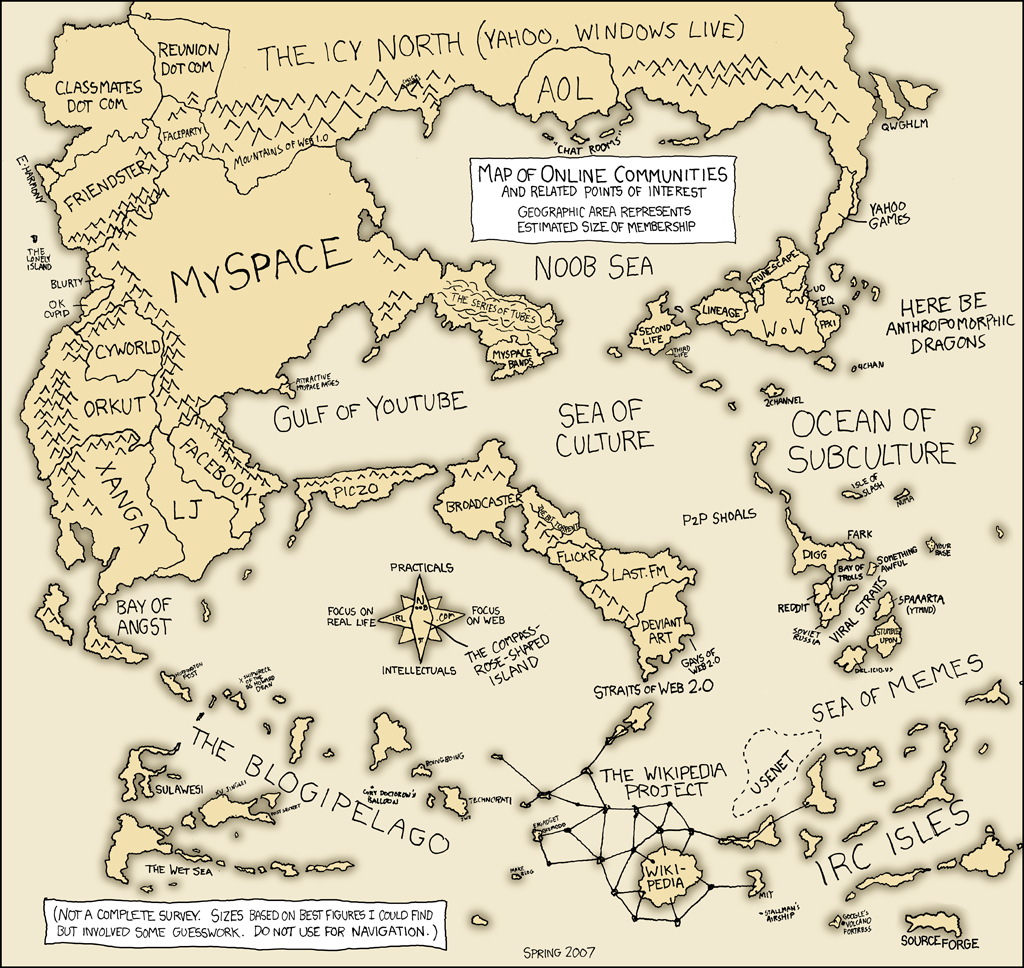
\includegraphics[height=\textheight]{../pics/online_communities}
\end{center}

\myslide{Map of online communities (2010)}
\MyLogo{\url{http://xkcd.com/802/} --- \href{https://www.explainxkcd.com/wiki/index.php/802}{explained!}}
\begin{center}
  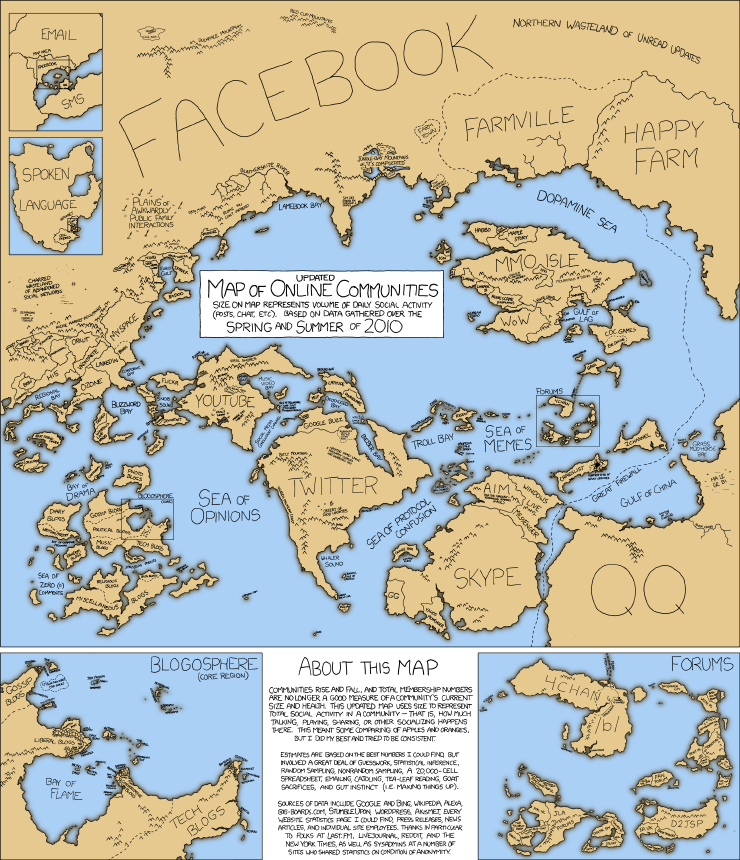
\includegraphics[height=\textheight]{../pics/online_communities_2}
\end{center}
%%% FIXME add date, newer map

\myslide{Growth of the Internet}
\begin{center}
  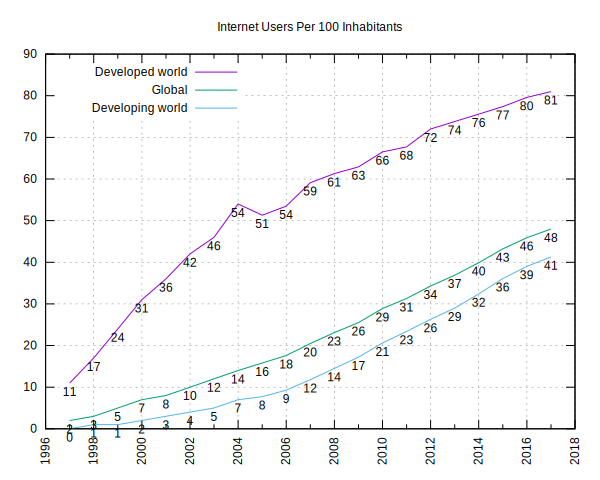
\includegraphics[height=0.9\textheight]{../pics/Internet_users_per_100_inhabitants_ITU}
\end{center}

In 2021: 63\% overall, 57\% developing, 90\% developed (\href{https://en.wikipedia.org/wiki/List_of_countries_by_number_of_Internet_users}{Wikipedia})

\MyLogo{\url{https://commons.wikimedia.org/wiki/File:Internet_users_per_100_inhabitants_ITU.svg}}

\section{Markup: \\ formatting information}

\myslide{Why Markup?}
\MyLogo{}

\begin{itemize}
\item \emp{Reduce Ambiguity}
  \begin{itemize}
  \item Need to make meaning explicit
  \end{itemize}
\item Traditionally this is done by annotating text in some way
\end{itemize}

\myslide{Markup Languages}

\begin{itemize}
\item Annotation on how to print is called \blu{markup}
  \begin{itemize}
  \item  underlining to indicate boldface
  \item special symbols for passages to be omitted
  \item special symbols for printed in a particular font
  \end{itemize}
\item This existed before computers
  \begin{itemize}
  \item Editors would markup hand-written manuscripts
  \item \ldots and pass them to type setters
  \item \ldots who would prepare the manuscript for printing
  \end{itemize}
\end{itemize}

\myslide{Printers' Markup}

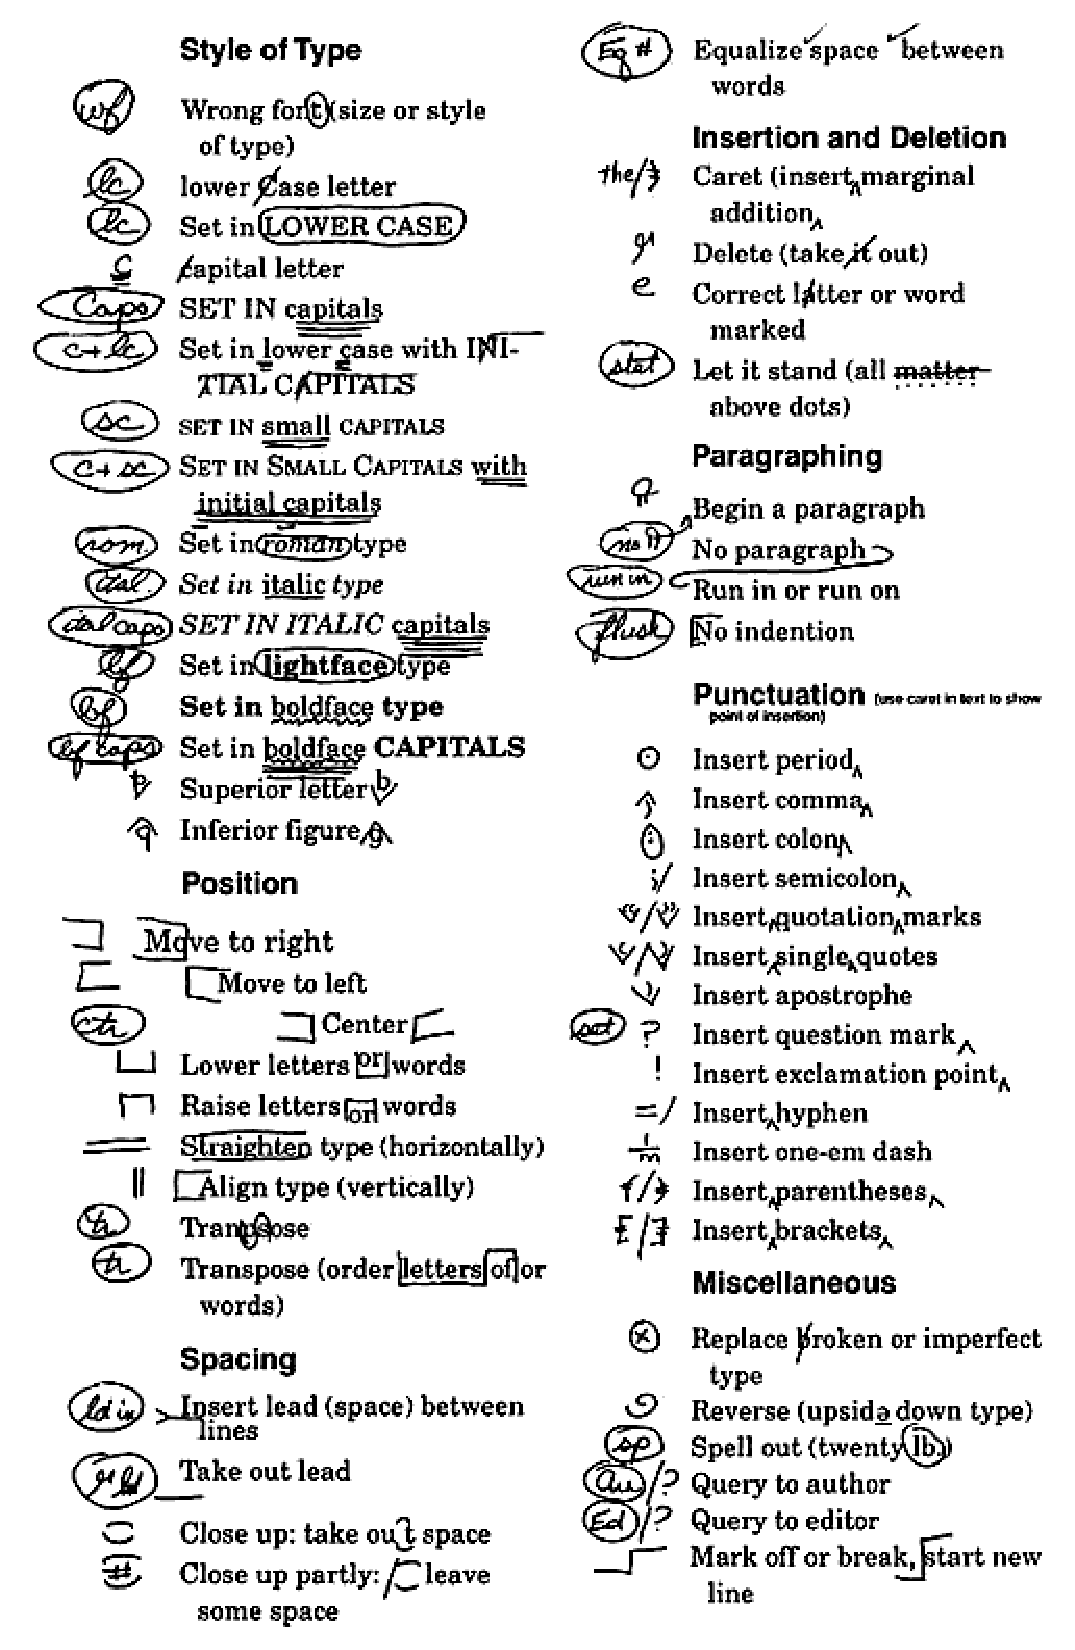
\includegraphics[trim= 0mm 188mm 0mm 0mm, clip=true, width=\textwidth]{../pics/proofreaders-marks.eps}


\myslide{Early Computer Markup (troff)}


\framebox{
  \begin{minipage}{0.5\linewidth}
\begin{flushleft}
  {\large \textbf{Headline}} \\
  and some text
\end{flushleft}
\end{minipage}}

\begin{verbatim}
.ps 12                         % point size 12
.ft B                          % font type Bold
Headline
.ps 10                         % point size 10
.ft R                          % font type Roman
and some text.
\end{verbatim} 

\begin{itemize}
\item   Marked up with \texttt{troff}
\item  Postscript and PDF (Portable Document Format) are similar
\end{itemize}


\myslide{Visual Markup vs Logical Markup}

\begin{itemize}
\item \txx{Visual Markup} (Presentational)
  \begin{itemize}
  \item What you see is what you get (\blu{WYSIWYG})
  \item Equivalent of printers' markup
  \item Shows what things look like
  \end{itemize}
\item \txx{Logical Markup} (Structural)
  \begin{itemize}
  \item Shows the structure and meaning
  \item Can be mapped to visual markup
  \item Less flexible than visual markup
  \item More adaptable (and reusable)
  \end{itemize}
\end{itemize}


\myslide{Standard Generalize Markup Language: SGML}

\begin{itemize}
\item ISO standard based on IBM's GML
\item Attempt to make markup independent of processor
  \begin{itemize}
  \item Important for archiving information
  \end{itemize}
\item Emphasis on logical markup\item Popularized the use of \url{<tag></tag>} notation
  \begin{itemize}
  \item and entities \url{&lt;} \url{&gt;} when you need an $< >$
  \end{itemize}
\item Split the document into: Declaration, Prolog, Documentation
\end{itemize}



\myslide{Hyper Text Markup Language: HTML}

\begin{itemize}
\item Markup Language for web pages
\item An extension of SGML
\item Combines logical and visual markup
\item Also allows hyperlinks (linking and anchoring)
\item Created by Tim Berners-Lee at CERN (1989)
  \begin{itemize}
  \item to make physics papers and documentation more accessible
  \end{itemize}
\end{itemize}



\myslide{HTML example}


\framebox{
  \begin{minipage}{0.5\linewidth}
\begin{flushleft}
  {\large \textbf{Headline}} \\
  and some text
\end{flushleft}
\end{minipage}}

\begin{itemize}
\item Logical
\begin{verbatim}
<h1>Headline</h1>
<p>and some text
\end{verbatim}

\item Visual
\begin{verbatim}
<font size="3"><b>Headline</b></font>
<br>and some text
\end{verbatim}
\end{itemize}

\myslide{Logical allows various styles}
\vspace*{1ex}
\framebox{
  \begin{minipage}{0.5\linewidth}
\begin{flushleft}
  {\large \blu{Headline}} \\[1.5ex]
  and some text
\end{flushleft}
\end{minipage}}


\begin{verbatim}
<style>
H1 {
           font-size:24px;
           color:blue;
           margin-top:10px;
           margin-bottom:15px;
      }
</style>
\end{verbatim}

\begin{itemize}\addtolength{\itemsep}{-1ex}
\item This can be done using CSS (Cascading Style Sheets)
\item Separate Logical and Visual Structure
\end{itemize}

\myslide{Benefits of Logical Tags}

\begin{itemize}
\item Can transform things easily
  \begin{itemize}
  \item No bold for Japanese and Chinese (just use size)
  \item Can adapt to other modalities (speech)
  \end{itemize}
\item Logical form useful for other tasks
  \begin{itemize}
  \item Summarization
    \begin{itemize}
    \item  Just show \texttt{<h1> \ldots\ <h3>}
    \end{itemize}
  \item Translation
    \begin{itemize}
    \item Headers are noun phrases, not sentences
    \end{itemize}
  \end{itemize}
\item Robustness: you can read the source directly
\end{itemize}


\myslide{But still there is ambiguity!}

\begin{itemize}
\item Tags on one site may not mean the same thing on another site
\item Huge amount of information
  \begin{itemize}
  \item Looking for \emp{Eric Miller} may get the wrong one!
  \item Looking for \emp{NTU} gets
    \begin{itemize}
    \item Nanyang Technological University
    \item National Taxpayers Union
    \item National Taiwan University
    \item Nottingham Trent University
    \end{itemize}
  \end{itemize}
\item What can we do?
\\ Semantic Web (week 10)
\end{itemize}

\myslide{Hypertext}

\begin{itemize}
\item HTML crucially adds \blu{hyperlinks}
  \begin{itemize}
  \item these extend text in a new way
  \item references that you can immediately access
  \end{itemize}
\item \texttt{<href="http://somewhere.on.the.web">link me</a>}
\item \texttt{<img src="http://somewhere.on.the.web/pic.jpg">}
\item Immediately accessible references are qualitatively different
\end{itemize}

\myslide{HTML example}
\begin{verbatim}
<!doctype html>
<html>
  <head>
    <title>Hello HTML</title>
  </head>
  <body>
    <p>Hello World!</p>
   <p>Oh well, <span lang="fr">c'est la vie</span>, 
      as they say in France.</p>
   <abbr id="anId" class="jargon" style="color:blue;" 
         title="Hypertext Markup Language">HTML</abbr>
  </body>
</html>
\end{verbatim}


\myslide{How should you hyperlink?}
\MyLogo{Inspired by \citet[p 28]{Crystal:2011}}

\begin{itemize}
\item Pick a page
  \begin{itemize}
  \item This course page
  \item The department's research page
  \item Wiki front page
  \item Your choice
  \end{itemize}
\item Discuss whether you think there are enough links or too many or
  not enough?  And are they linking to the best targets?
\item You may wish to look at the \textit{Wikipedia:Manual of Style/Linking}
\\ \url{<https://en.wikipedia.org/wiki/Wikipedia:Manual_of_Style/Linking>}
\end{itemize}


\myslide{The Structure of the Web}
\MyLogo{\url{https://en.wikipedia.org/wiki/World_Wide_Web}}

\begin{itemize}
\item 550 billion documents on the Web (2001)
  \\ mostly in the invisible Web, or deep Web
\item 11.5 billion indexable web pages (2005)
\item 25.21 billion indexable web pages (2009)
\item 109.5 million websites (2009)
\item 5.9 billion indexed pages (Sunday, 23 February, 2020).
  \\ 60 billion pages (googles index)
\item  3.21 billion indexed pages (Monday, 23 October, 2023).
    \\ 50 billion pages (googles index)
  \\ \url{https://www.worldwidewebsize.com/}
\end{itemize}

\myslide{The Deep Web}
\begin{description}
\item [Dynamic content] dynamic pages which are returned in response to a submitted query or accessed only through a form
\item [Unlinked content] pages which are not linked to by other pages (but clicking links them)
\item [Private Web] sites that require registration and login
  \com{Edventure, NTULearn}
\item [Contextual Web] pages with content varying for different access contexts (e.g., ranges of client IP addresses or previous navigation sequence).
\item [Limited access content] sites that limit access to their pages
  in a technical way (e.g., using the Robots Exclusion Standard)
\item [Scripted content] pages that are only accessible through links produced by JavaScript as well as content dynamically downloaded from Web servers via Flash or Ajax solutions.
\item [Non-HTML/text content] textual content encoded in multimedia (image or video) files or specific file formats not handled by search engines.
\end{description}

These pages all include data that search engines cannot find!

\myslide{robots.txt}
\MyLogo{\url{http://www.robotstxt.org}}
\begin{itemize}
\item A \blu{Robot} (Web Crawler, or Spiders) is a program that
  automatically traverses the Web's hypertext structure by retrieving
  a document, and recursively retrieving all documents that are
  referenced. Robots are used for:
  \begin{itemize}
  \item Indexing and \textit{What's New} monitoring
  \item HTML and Link validation  
  \item Mirroring and back up
  \end{itemize}
\item A website can explicitly tell robots where they can and cannot go
  \begin{itemize}
  \item Compliance is voluntary, but followed by most robots
  \end{itemize}
\item You can \blu{Allow} and \blu{Disallow} whole directories, or individual pages
\item You can \blu{Allow} and \blu{Disallow} individual user-agents
  (such as \texttt{Google} or \texttt{ChatGPT})
  \\ For example to disallow OpenAI's crawler (for ChatGPT): 
\begin{verbatim}
User-agent: GPTBot
Disallow: /
\end{verbatim}
\end{itemize}


\myslide{The Internet and Language Diversity}
%%% FIXME add more from Crystal
\MyLogo{}
\begin{center}
  \includegraphics[height=\textheight]{../pics/web-users.eps}
\end{center}

\myslide{Distribution of languages among Internet users }
\MyLogo{From Global Reach (2006) cited in Gerrand (2007)}
\begin{center}
  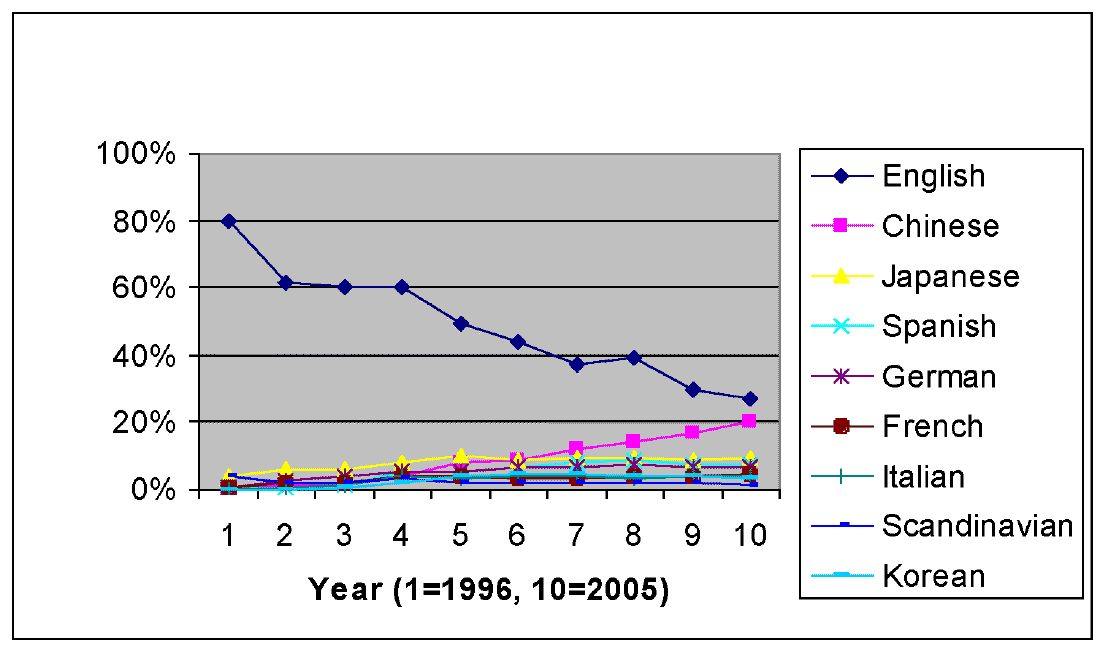
\includegraphics[width=0.9\textwidth]{../pics/gerrand.fig5.jpg}
\end{center}

\myslide{Internet users by language, February 2005}
\MyLogo{Source: OECD (2006)  cited in Gerrand (2007)} 
\begin{center}
  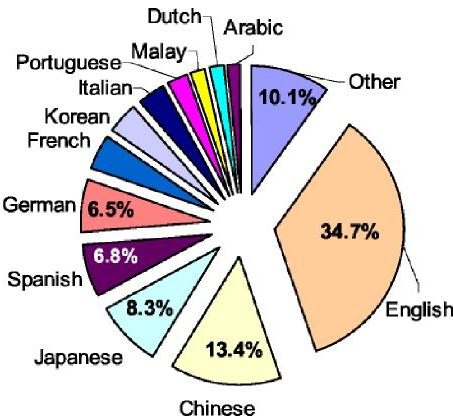
\includegraphics[height=0.9\textheight]{../pics/gerrand.fig6b.jpg}
\end{center}


\myslide{Language of e-commerce, February 2005}

\begin{center}
  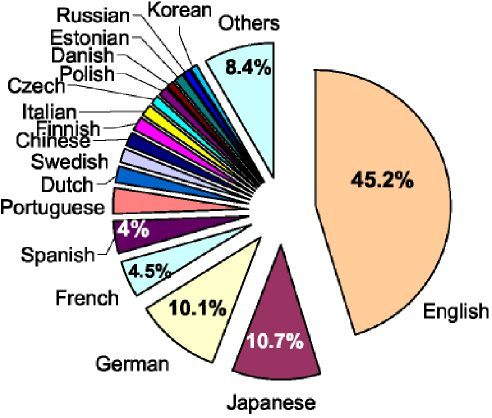
\includegraphics[height=0.9\textheight]{../pics/gerrand.fig6a.jpg}
\end{center}

\MyLogo{Source: OECD (2006) references to secure servers by language  cited in Gerrand (2007)} 



\myslide{Percentage of Web sites by language (2014)}
\MyLogo{\url{https://en.wikipedia.org/wiki/Languages_used_on_the_Internet}}
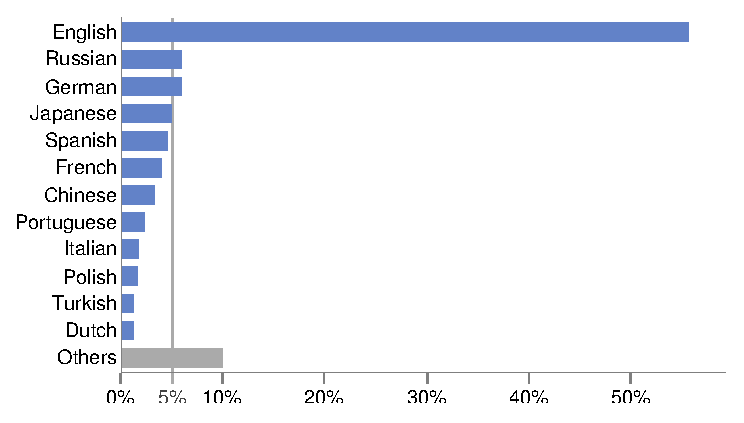
\includegraphics[height=0.9\textheight]{../pics/WebsiteContentLanguages}

\myslide{Percentage of Web users by language (2014)}
\MyLogo{\url{https://en.wikipedia.org/wiki/Languages_used_on_the_Internet}}
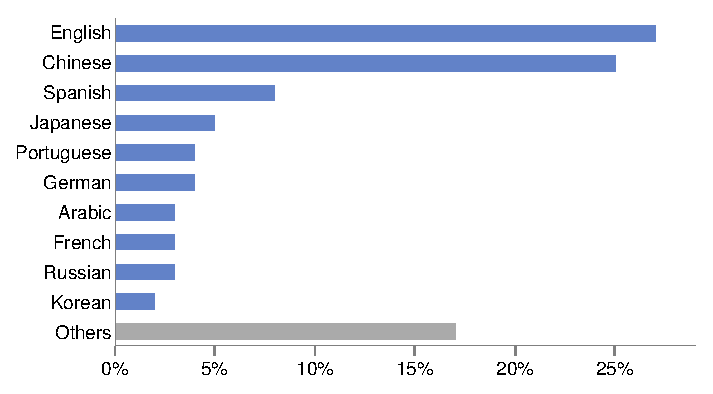
\includegraphics[height=0.9\textheight]{../pics/WebsiteUserLanguageBars}

\myslide{Gradually  Changing}
\MyLogo{\url{https://www.internetworldstats.com/stats7.htm}}
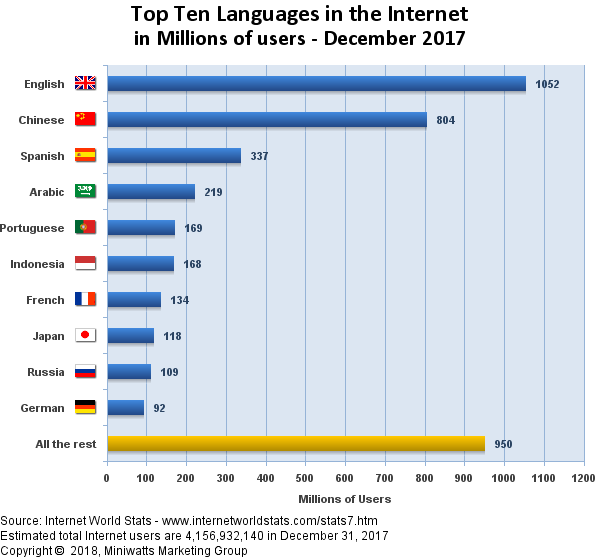
\includegraphics[height=\textheight]{../pics/languages2017Q4.png}


\myslide{The Internet and Language Diversity}
\MyLogo{}
\begin{itemize}
\item Major languages will survive (not just English)
\item \textbf{Sarnoff's Law:} the value of a broadcast network is
  proportional to the number of viewers ($n$)
\item \textbf{Metcalfe's Law:} the value of a telecommunications
    network is proportional to the square of the number of connected
    users of the system ($n^2$)
    \begin{itemize}
    \item[$\Rightarrow$] languages with more pages will become even more valuable
    \end{itemize}
\item Minor languages probably won't survive
\end{itemize}




\myslide{Top ten Wikipedias}
\MyLogo{\url{http://en.wikipedia.org/wiki/Wikipedia:Size_of_Wikipedia}}
\begin{center}
  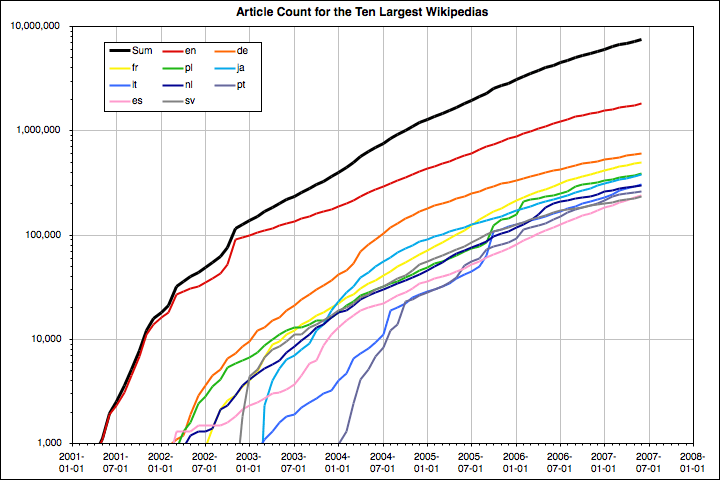
\includegraphics[height=0.8\textheight]{../pics/TopTenWikipediasGraph}
\end{center}
 See also \url{http://meta.wikimedia.org/wiki/List_of_Wikipedias}
\\ Wikipedias in 272 languages: only 96 with more than 10,000 pages

\myslide{The next 5,000 days of the Web}
\MyLogo{}
\begin{itemize}
\item Kevin Kelly on the next 5,000 days of the web (2007)
\item
  \url{https://www.ted.com/talks/kevin_kelly_the_next_5_000_days_of_the_web}
  (20min)
\item The impossible has become possible
\item The web is a single machine
  \begin{itemize}
  \item Embodiment
  \item Re-structuring
  \item Co-dependence
  \end{itemize}
\item The future will be shaped by optimists (Kevin Kelly, 2021)
\item \url{https://www.ted.com/talks/kevin_kelly_the_future_will_be_shaped_by_optimists} (10min)

\end{itemize}

\myslide{Linguistic features of the web}

\begin{itemize}
\item Much/most text is just the same
\item Un-edited
\item Accessible in great volume (and many languages)
\item Editable --- Wikis, comments, tweets
\item Multi-media
\end{itemize}

\myslide{Conclusion}

\begin{itemize}
\item The web is changing what humanity can do with language
\item It is not clear if it is changing what individual humans do
\bigskip
\item \href{https://en.wikipedia.org/wiki/Wikipedia:Tutorial}{Make sure you go through the wikipedia tutorial}
\end{itemize}



\myslide{References}

\begin{itemize}
\item \bibentry{Crystal:2011}
\item Peter Gerrand (2007) Estimating linguistic diversity on the
  Internet: A taxonomy to avoid pitfalls and
  paradoxes. \textit{Journal of Computer-Mediated Communication},
  12(4), article
  8. \url{http://jcmc.indiana.edu/vol12/issue4/gerrand.html}
\item Global Reach. (2006). Global Internet Statistics (by
  Language). Retrieved October 11, 2006 from
  \url{http://www.global-reach.biz/globstats/index.php3}
\end{itemize}

%% 
%% Future
%%
\end{document}



%%% Local Variables: 
%%% coding: utf-8
%%% mode: latex
%%% TeX-PDF-mode: t
%%% TeX-engine: xetex
%%% End: 
